% Options for packages loaded elsewhere
\PassOptionsToPackage{unicode}{hyperref}
\PassOptionsToPackage{hyphens}{url}
%
\documentclass[
]{article}
\usepackage{amsmath,amssymb}
\usepackage{lmodern}
\usepackage{iftex}
\ifPDFTeX
  \usepackage[T1]{fontenc}
  \usepackage[utf8]{inputenc}
  \usepackage{textcomp} % provide euro and other symbols
\else % if luatex or xetex
  \usepackage{unicode-math}
  \defaultfontfeatures{Scale=MatchLowercase}
  \defaultfontfeatures[\rmfamily]{Ligatures=TeX,Scale=1}
\fi
% Use upquote if available, for straight quotes in verbatim environments
\IfFileExists{upquote.sty}{\usepackage{upquote}}{}
\IfFileExists{microtype.sty}{% use microtype if available
  \usepackage[]{microtype}
  \UseMicrotypeSet[protrusion]{basicmath} % disable protrusion for tt fonts
}{}
\makeatletter
\@ifundefined{KOMAClassName}{% if non-KOMA class
  \IfFileExists{parskip.sty}{%
    \usepackage{parskip}
  }{% else
    \setlength{\parindent}{0pt}
    \setlength{\parskip}{6pt plus 2pt minus 1pt}}
}{% if KOMA class
  \KOMAoptions{parskip=half}}
\makeatother
\usepackage{xcolor}
\usepackage[margin=1in]{geometry}
\usepackage{graphicx}
\makeatletter
\def\maxwidth{\ifdim\Gin@nat@width>\linewidth\linewidth\else\Gin@nat@width\fi}
\def\maxheight{\ifdim\Gin@nat@height>\textheight\textheight\else\Gin@nat@height\fi}
\makeatother
% Scale images if necessary, so that they will not overflow the page
% margins by default, and it is still possible to overwrite the defaults
% using explicit options in \includegraphics[width, height, ...]{}
\setkeys{Gin}{width=\maxwidth,height=\maxheight,keepaspectratio}
% Set default figure placement to htbp
\makeatletter
\def\fps@figure{htbp}
\makeatother
\setlength{\emergencystretch}{3em} % prevent overfull lines
\providecommand{\tightlist}{%
  \setlength{\itemsep}{0pt}\setlength{\parskip}{0pt}}
\setcounter{secnumdepth}{-\maxdimen} % remove section numbering
\ifLuaTeX
  \usepackage{selnolig}  % disable illegal ligatures
\fi
\IfFileExists{bookmark.sty}{\usepackage{bookmark}}{\usepackage{hyperref}}
\IfFileExists{xurl.sty}{\usepackage{xurl}}{} % add URL line breaks if available
\urlstyle{same} % disable monospaced font for URLs
\hypersetup{
  pdftitle={CH1-5},
  hidelinks,
  pdfcreator={LaTeX via pandoc}}

\title{CH1-5}
\author{}
\date{\vspace{-2.5em}2024-03-09}

\begin{document}
\maketitle

\hypertarget{the-penguins-data-frame}{%
\section{1: The penguins data frame}\label{the-penguins-data-frame}}

You can see all variables and the first few observations of each
variable by using \texttt{glimpse()}.

\begin{verbatim}
## Rows: 344
## Columns: 8
## $ species           <fct> Adelie, Adelie, Adelie, Adelie, Adelie, Adelie, Adel~
## $ island            <fct> Torgersen, Torgersen, Torgersen, Torgersen, Torgerse~
## $ bill_length_mm    <dbl> 39.1, 39.5, 40.3, NA, 36.7, 39.3, 38.9, 39.2, 34.1, ~
## $ bill_depth_mm     <dbl> 18.7, 17.4, 18.0, NA, 19.3, 20.6, 17.8, 19.6, 18.1, ~
## $ flipper_length_mm <int> 181, 186, 195, NA, 193, 190, 181, 195, 193, 190, 186~
## $ body_mass_g       <int> 3750, 3800, 3250, NA, 3450, 3650, 3625, 4675, 3475, ~
## $ sex               <fct> male, female, female, NA, female, male, female, male~
## $ year              <int> 2007, 2007, 2007, 2007, 2007, 2007, 2007, 2007, 2007~
\end{verbatim}

\hypertarget{creating-a-ggplot}{%
\section{2: Creating a ggplot}\label{creating-a-ggplot}}

The \texttt{mapping} argument of the \texttt{ggplot()} function defines
how variables in your dataset are mapped to visual properties
(\emph{aesthetics}) of your plot. The \texttt{mapping} argument is
always defined in the \texttt{aes()} function, and the \texttt{x} and
\texttt{y} arguments of \texttt{aes()} specify which variables to map to
the x and y axes.

\emph{geom:} The geometrical object that a plot uses to represent data.
These geometric objects are made available in ggplot2 with functions
that start with \texttt{geom\_}.

People often describe plots by the type of geom that the plot uses. For
example, bar charts use bar geoms (\texttt{geom\_bar()}), line charts
use line geoms (\texttt{geom\_line()}), boxplots use boxplot geoms
(\texttt{geom\_boxplot()}), scatterplots use point geoms
(\texttt{geom\_point()}), and so on.

The function \texttt{geom\_point()} adds a layer of points to your plot,
which creates a scatterplot.

When a categorical variable is mapped to an aesthetic, ggplot2 will
automatically assign a unique value of the aesthetic (here a unique
color) to each unique level of the variable (each of the three species),
a process known as \emph{scaling}. ggplot2 will also add a legend that
explains which values correspond to which levels.

Now let's add one more layer: a smooth curve displaying the relationship
between body mass and flipper length.Since this is a new geometric
object representing our data, we will add a new geom as a layer on top
of our point geom: \texttt{geom\_smooth()}. And we will specify that we
want to draw the line of best fit based on a \texttt{l}inear
\texttt{m}odel with \texttt{method\ =\ "lm"}.

\begin{verbatim}
## `geom_smooth()` using formula = 'y ~ x'
\end{verbatim}

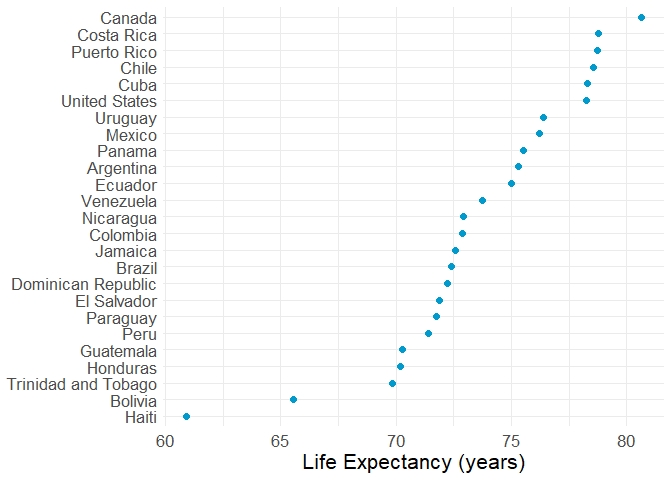
\includegraphics{CH1-5_files/figure-latex/unnamed-chunk-3-1.pdf}

When aesthetic mappings are defined in \texttt{ggplot()}, at the global
level, they're passed down to each of the subsequent geom layers of the
plot. However, each geom function in ggplot2 can also take a
\texttt{mapping} argument, which allows for aesthetic mappings at the
local level that are added to those inherited from the global level.

Since we want points to be colored based on species but don't want the
lines to be separated out for them, we should specify
\texttt{color\ =\ species} for \texttt{geom\_point()} only.

It's generally not a good idea to represent information using only
colors on a plot, as people perceive colors differently due to color
blindness or other color vision differences. Therefore, in addition to
color, we can also map \texttt{species} to the \texttt{shape} aesthetic.

\begin{verbatim}
## `geom_smooth()` using formula = 'y ~ x'
\end{verbatim}

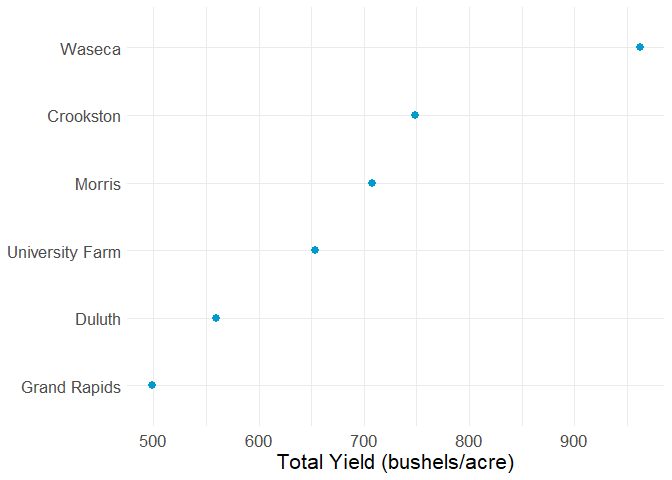
\includegraphics{CH1-5_files/figure-latex/unnamed-chunk-4-1.pdf}

We can improve the labels of our plot using the \texttt{labs()} function
in a new layer. Some of the arguments to \texttt{labs()} might be self
explanatory: title adds a \texttt{title} and subtitle adds a
\texttt{subtitle} to the plot. Other arguments match the aesthetic
mappings, \texttt{x} is the x-axis label, \texttt{y} is the y-axis
label, and \texttt{color} and \texttt{shape} define the label for the
legend. In addition, we can improve the color palette to be colorblind
safe with the \texttt{scale\_color\_colorblind()} function from the
\texttt{ggthemes} package.

\begin{verbatim}
## `geom_smooth()` using formula = 'y ~ x'
\end{verbatim}

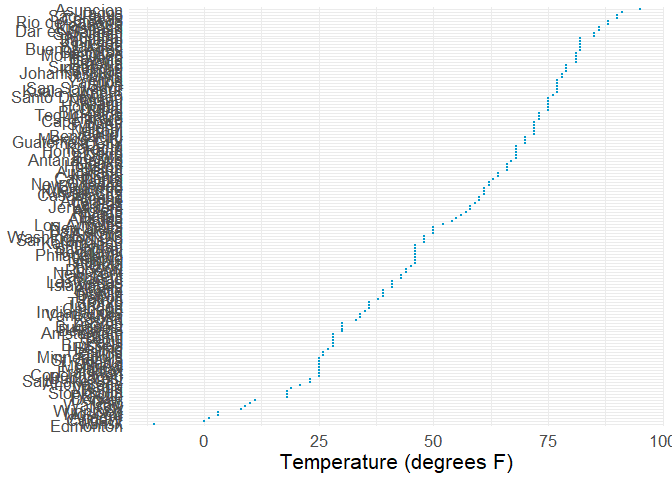
\includegraphics{CH1-5_files/figure-latex/unnamed-chunk-5-1.pdf}

\hypertarget{visualizing-distributions}{%
\section{3. Visualizing distributions}\label{visualizing-distributions}}

A variable is \emph{categorical} if it can only take one of a small set
of values. To examine the distribution of a categorical variable, you
can use a bar chart. The height of the bars displays how many
observations occurred with each x value.

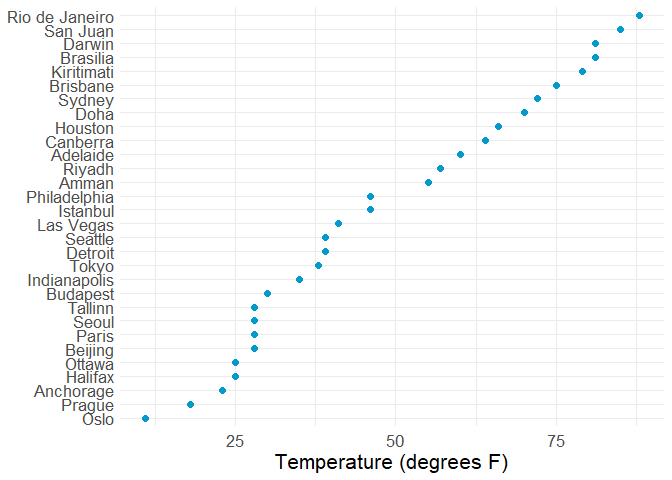
\includegraphics{CH1-5_files/figure-latex/unnamed-chunk-6-1.pdf}

In bar plots of categorical variables with non-ordered levels, like the
penguin species above, it's often preferable to reorder the bars based
on their frequencies. Doing so requires transforming the variable to a
factor (how R handles categorical data) and then reordering the levels
of that factor. So, you can use \texttt{fct\_infreq()}.

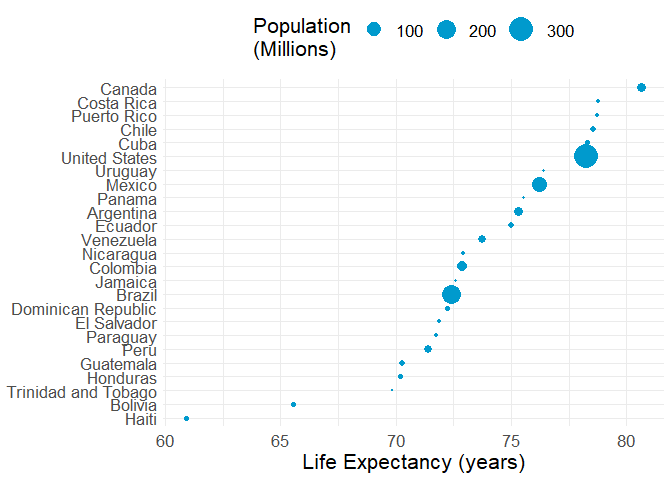
\includegraphics{CH1-5_files/figure-latex/unnamed-chunk-7-1.pdf}

A variable is \emph{numerical} (or quantitative) if it can take on a
wide range of numerical values, and it is sensible to add, subtract, or
take averages with those values. Numerical variables can be continuous
or discrete.

One commonly used visualization for distributions of continuous
variables is a \emph{histogram}. A histogram divides the x-axis into
equally spaced bins and then uses the height of a bar to display the
number of observations that fall in each bin.

You can set the width of the intervals in a histogram with the binwidth
argument, which is measured in the units of the x variable.

\includegraphics{CH1-5_files/figure-latex/unnamed-chunk-8-1.pdf}

You should always explore a variety of binwidths when working with
histograms, as different binwidths can reveal different patterns.

In the plots below a binwidth of 20 is too narrow, resulting in too many
bars, making it difficult to determine the shape of the distribution.
Similarly, a binwidth of 2,000 is too high, resulting in all data being
binned into only three bars, and also making it difficult to determine
the shape of the distribution.

\includegraphics{CH1-5_files/figure-latex/unnamed-chunk-9-1.pdf}
\includegraphics{CH1-5_files/figure-latex/unnamed-chunk-9-2.pdf}

A \emph{density} plot is a smoothed-out version of a histogram and a
practical alternative, particularly for continuous data that comes from
an underlying smooth distribution.

\includegraphics{CH1-5_files/figure-latex/unnamed-chunk-10-1.pdf}

\hypertarget{visualizing-relationships}{%
\section{4. Visualizing relationships}\label{visualizing-relationships}}

To visualize the relationship between a \emph{numerical} and a
\emph{categorical} variable we can use side-by-side box plots.

A \emph{boxplot} is a type of visual shorthand for measures of position
(percentiles) that describe a distribution. It is also useful for
identifying potential outliers.

\begin{itemize}
\item
  A box that indicates the range of the middle half of the data, a
  distance known as the interquartile range (IQR). The 25th, 75th, and
  the median lines give you a sense of the spread of the distribution
  and whether or not the distribution is symmetric about the median or
  skewed to one side.
\item
  A line (or whisker) that extends from each end of the box and goes to
  the farthest non-outlier point in the distribution.
\end{itemize}

\includegraphics{CH1-5_files/figure-latex/unnamed-chunk-11-1.pdf}
Alternatively, we can make density plots with \texttt{geom\_density()}.
You can customize the thickness of the lines using the
\texttt{linewidth} argument in order to make them stand out a bit more
against the background.

\includegraphics{CH1-5_files/figure-latex/unnamed-chunk-12-1.pdf}
Additionally, we can map species to both \texttt{color} and
\texttt{fill} aesthetics and use the \texttt{alpha} aesthetic to add
transparency to the filled density curves. This aesthetic takes values
between 0 (completely transparent) and 1 (completely opaque).

\includegraphics{CH1-5_files/figure-latex/unnamed-chunk-13-1.pdf}

We can use \texttt{stacked\ bar\ plots} to visualize the relationship
between two categorical variables.

The first plot shows the frequencies of each species of penguins on each
island. The plot of frequencies shows that there are equal numbers of
Adelies on each island. But we don't have a good sense of the percentage
balance within each island.

\includegraphics{CH1-5_files/figure-latex/unnamed-chunk-14-1.pdf} The
second plot, a relative frequency plot created by setting
\texttt{position\ =\ "fill"} in the geom, is more useful for comparing
species distributions across islands since it's not affected by the
unequal numbers of penguins across the islands.

Using this plot we can see that Gentoo penguins all live on Biscoe
island and make up roughly 75\% of the penguins on that island,
Chinstrap all live on Dream island and make up roughly 50\% of the
penguins on that island, and Adelie live on all three islands and make
up all of the penguins on Torgersen.

In creating these bar charts, we map the variable that will be separated
into bars to the \texttt{x} aesthetic, and the variable that will change
the colors inside the bars to the \texttt{fill} aesthetic.

\includegraphics{CH1-5_files/figure-latex/unnamed-chunk-15-1.pdf}

\hypertarget{three-or-more-variables}{%
\section{5. Three or more variables}\label{three-or-more-variables}}

We can incorporate more variables into a plot by mapping them to
additional aesthetics. For example, in the following scatterplot the
colors of points represent species and the shapes of points represent
islands.

\includegraphics{CH1-5_files/figure-latex/unnamed-chunk-16-1.pdf}

However adding too many aesthetic mappings to a plot makes it cluttered
and difficult to make sense of. Another way, which is particularly
useful for categorical variables, is to split your plot into
\emph{facets}, subplots that each display one subset of the data.

To facet your plot by a single variable, use \texttt{facet\_wrap()}. The
first argument of \texttt{facet\_wrap()} is a formula, which you create
with \texttt{\textasciitilde{}} followed by a variable name. The
variable that you pass to \texttt{facet\_wrap()} should be
\emph{categorical}.

\includegraphics{CH1-5_files/figure-latex/unnamed-chunk-17-1.pdf}

\end{document}
